\subsection{What}\label{what}
\begin{center}

\textit{Cosa offre il sito?}

\end{center}
\begin{flushleft}
Questo asse non è subito visualizzabile in modo chiaro, solo effetuando un 
primo scroll è possibile capire quali siano gli strumenti di analisi web
che effettivamente il sito offre.
Ciò si sarebbe potuto evitare riorganizzando lo spazio della prima pagina senza scroll
o ampliandolo alle colonne laterali che non vengono mai utilizzate nella homepage.
Inoltre, le informazioni riguardanti l'asse \textit{What} non sono sempre organizzate in modo standard in 
tutte le pagine di scroll presenti in homepage:
\begin{itemize}
	\item la prima pagina di scroll utile le organizza a griglia;
	\item la seconda le dispone orizzontalmente;
	\item dalla terza pagina verticalmente (implica ulteriore scroll);
	\item dalla quinta di nuovo orizzontalmente fino all'ultima.
\end{itemize}
Queste diverse disposizioni
affaticano l'utente nella navigazione della homepage. \\
Screenshot disponibile al path : \textit{figure/3/what0.png} \\
Un'altra osservazione
riguarda le immagini, in questo caso viene violata una convenzione web importante: 
\begin{center}
	le immagini devono essere cliccabili
\end{center}
Non tutte le immagini riguardanti l'asse \textit{What} sono cliccabili, l'unico modo 
di accedere alle funzionalità presentate è utilizzare il pulsante correlato 
che almeno risulta ben visibile e correttamente implementato (la zona cliccabile corrisponde a 
tutta la zona visibile). Le informazioni, anche se presentate in modo non ottimale,
risultano tuttavia esaustive.
    \begin{figure}[ht]
    \centering
    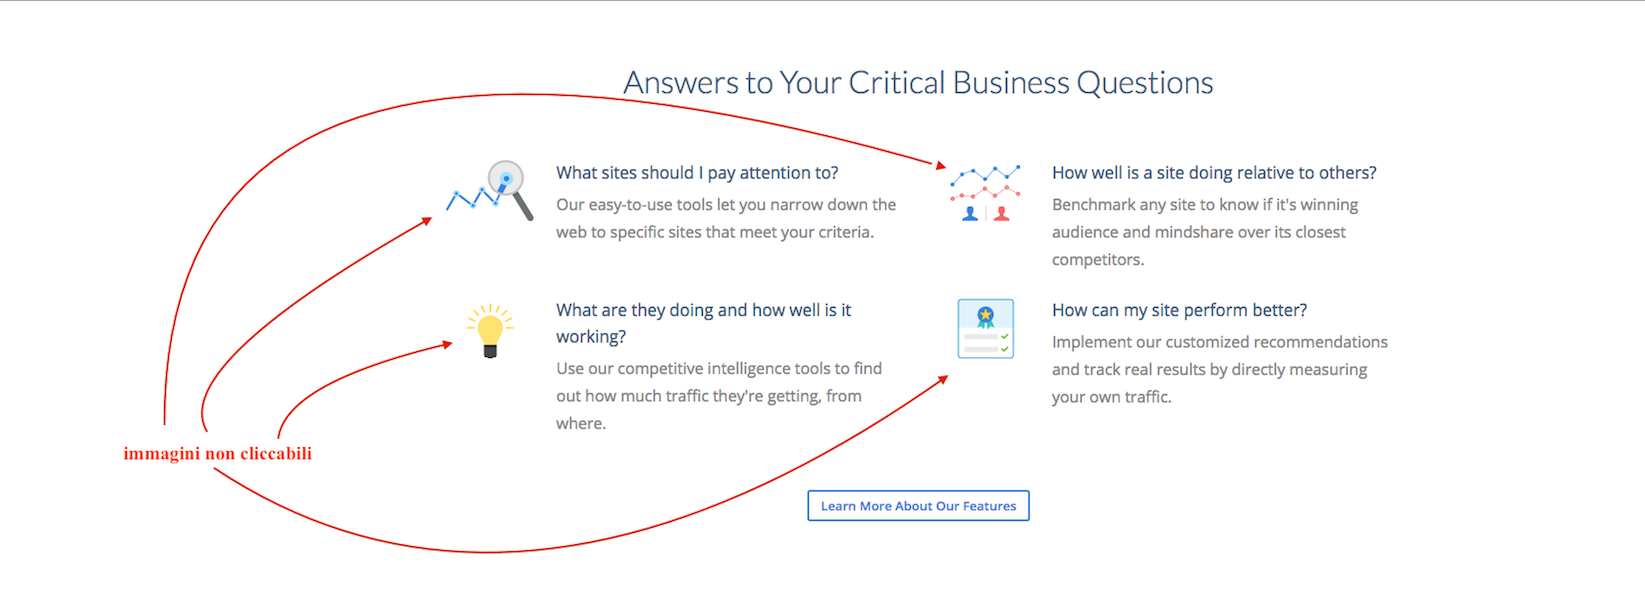
\includegraphics[scale=0.28,keepaspectratio]{{figure/3/what1}.png}
    \caption{Homepage - immagini non cliccabili}
    \end{figure}
    \FloatBarrier 
Risultato : \textit{6}
\end{flushleft}